\documentclass[11pt]{article}
\usepackage[a4paper,margin=2cm]{geometry}
\usepackage{amsmath,amssymb}
\usepackage{graphicx}
\usepackage{booktabs}
\usepackage{float}
\usepackage{caption}
\usepackage[dvipsnames]{xcolor}
\usepackage[colorlinks=true,linkcolor=blue!50!black,citecolor=blue!50!black,urlcolor=blue!50!black]{hyperref}
\captionsetup{font=small,labelfont=bf}
\graphicspath{{../../data/plots/2026-11-03_ksz_lae_snr/}}
\newcommand{\kSZ}{\mathrm{kSZ}}
\newcommand{\LP}{La~Plante+22}

\title{kSZ$^2\times$LAE cross-correlation: signal-to-noise pipeline,\\ validation against La~Plante et al.\ (2022), and detectability\\ for current and future CMB and LAE surveys}
\author{Swanith Upadhye (TIFR)}
\date{4 November 2026}

\begin{document}
\maketitle

\section*{Summary}
\begin{itemize}
\item We forecast the signal-to-noise (S/N) of the cross-correlation between the filtered and squared CMB temperature map (the kSZ$^2$ map) and Lyman-$\alpha$ emitters (LAEs), with the estimator of \LP\ (their Eq.~13). The CMB noise, the LAE shot noise and the sample (cosmic) variance are all included (Sec.~\ref{sec:estimator}).
\item The signal comes from our simulation (21cmFAST v4, ten 300\,Mpc boxes): either La~Plante's galaxy model (matter $\times$ Waters+16 bias) or the simulated LAEs, rescaled to each survey's bias (Sec.~\ref{sec:signal}).
\item \textbf{Validation} (Sec.~\ref{sec:validation}). On La~Plante's exact setup our noise matches theirs bin by bin and our galaxy clustering matches their Fig.~8. Our total S/N is 0.7--0.85 of their Table~2 with shot noise. The gap comes from the modes our box does not contain ($\ell \lesssim 240$) and from a signal about two times lower at $\ell\gtrsim1000$ (not yet explained).
\item \textbf{Detectability} (Sec.~\ref{sec:pairs}). None of the requested CMB$\times$LAE pairs reaches 1$\sigma$ with the validated signal model. Existing data (ACT DR6 $\times$ SILVERRUSH) give $\sim$0.01. A better CMB alone (SO LAT) does not help, because the LAE fields are only 10--20\,deg$^2$. CMB-HD $\times$ a 1\,deg$^2$ Roman deep field reaches 0.04--0.2 (0.2--1.2 with the simulated-LAE signal, whose excess is not yet confirmed). A 3$\sigma$ detection with CMB-HD needs Roman-deep-quality LAEs over $\sim$200--7000\,deg$^2$.
\end{itemize}

\section{Estimator}\label{sec:estimator}
\paragraph{S/N.} Following \LP\ (Eq.~13; Gaussian approximation, after Ferraro et al.\ 2016), for one galaxy redshift window
\begin{equation}
\left(\frac{S}{N}\right)^2 = f_{\rm sky}\sum_{\ell=\ell_{\min}}^{\ell_{\max}} \frac{(2\ell+1)\,\bigl(C_\ell^{\kSZ^2\times g}\bigr)^2}{C^{T^2T^2}_{f}\,C_\ell^{gg} + \bigl(C_\ell^{\kSZ^2\times g}\bigr)^2},
\qquad \ell_{\max}=10^4 .
\label{eq:snr}
\end{equation}
The three noise sources enter as follows: the CMB noise through $C^{T^2T^2}_f$; the LAE shot noise through the Poisson part of $C^{gg}_\ell$; and the sample variance through the clustering part of $C^{gg}_\ell$, the $(C_\ell^{\kSZ^2\times g})^2$ term, and the finite number of modes $f_{\rm sky}(2\ell+1)$.
The spectra are binned in $\ell$, so the sum over a bin uses $\sum_{\ell\in{\rm bin}}(2\ell+1)\simeq \ell_{\rm hi}^2-\ell_{\rm lo}^2$. Several redshift shells of one survey are combined in quadrature.

\paragraph{CMB filter} (\LP\ Eqs.~8, 10):
\begin{equation}
f(\ell) \propto F(\ell)\,b(\ell),\qquad
F(\ell)=\frac{C_\ell^{\kSZ,{\rm reion}}}{C_\ell^{TT}+C_\ell^{\kSZ,{\rm reion}}+C_\ell^{\kSZ,{\rm late}}+N_\ell},\qquad
b(\ell)=e^{-\theta^2\ell^2/(16\ln2)},
\end{equation}
with $\theta$ the beam FWHM. $f$ is normalised to 1 at its peak (as in \LP\ Fig.~2); the S/N does not depend on this normalisation because signal and noise use the same $f$.

\paragraph{Noise of the filtered, squared map} (\LP\ Eqs.~14--15):
\begin{equation}
C^{T^2T^2}_f = 2\int\frac{\ell\,{\rm d}\ell}{2\pi}\Bigl[C^{\bar T\bar T,f}_\ell\Bigr]^2,\qquad
C^{\bar T\bar T,f}_\ell = f(\ell)^2\bigl(C_\ell^{TT}+C_\ell^{\kSZ,{\rm reion}}+C_\ell^{\kSZ,{\rm late}}+N_\ell\bigr).
\end{equation}
\paragraph{CMB noise $N_\ell$.} Two cases:
\begin{align}
\text{instrument only (\LP\ Eq.~11):}\quad & N_\ell = \Delta_T^2\,e^{\theta^2\ell^2/(8\ln2)},\\
\text{post-ILC:}\quad & N_\ell = N_\ell^{\rm ILC}\quad\text{(\LP\ Fig.~1)}.
\end{align}
$N_\ell^{\rm ILC}$ is the instrument noise plus the residual foregrounds after the internal linear combination of the frequency channels. Post-ILC curves exist only for SO, CMB-S4 and CMB-HD. ACT DR6 and SPT-3G are therefore used with instrument noise only, which is optimistic.

\paragraph{Galaxy auto-power} (\LP\ Eq.~16):
\begin{equation}
C_\ell^{gg}=C_\ell^{\rm clust}+C^{\rm SN},\qquad C^{\rm SN}=\frac{1}{\bar n_{2D}}=\frac{4\pi f_{\rm sky}}{N_g},
\end{equation}
with $\bar n_{2D}$ the number of LAEs per steradian in the shell.

\paragraph{LAE number density.} From a Schechter fit to the observed Ly$\alpha$ luminosity function (LF), per dex,
\begin{equation}
n_{3D}(>L_{\min})=\int_{\log L_{\min}}\! \ln10\,\phi^*\Bigl(\frac{L}{L^*}\Bigr)^{\alpha+1} e^{-L/L^*}\,{\rm d}\log L,\qquad
\bar n_{2D}=n_{3D}\,\chi^2\Delta\chi .
\end{equation}
Where a survey's catalogue count is published, the shot noise uses that count instead (Table~\ref{tab:lae}). The survey bias always uses $n_{3D}$ from the LF: incompleteness thins the sample at random and does not change its bias.

\paragraph{Survey bias.} We use abundance matching: we find $M_{\min}$ with $n_{\rm ST}(>M_{\min},z)=n_{3D}$ and set $b_{\rm survey}=b_{\rm SMT}(M_{\min},z)$. Here $n_{\rm ST}$ is the Sheth \& Tormen (1999) mass function, $b_{\rm SMT}$ is the Sheth, Mo \& Tormen (2001) bias, and $\sigma(M)$ uses the Eisenstein \& Hu (1998) transfer function. This is an upper value (no scatter, no duty cycle). For the validation we use La~Plante's bias instead, $b_g(z)=2.1(1+z)-5.3$ (Waters et al.\ 2016, Sec.~5, Fig.~14).

\paragraph{Smallest usable multipole.} A field of solid angle $\Omega$ cannot measure modes larger than itself, so
\begin{equation}
\ell_{\min}=\max\bigl(100,\ 2\pi/\sqrt{\Omega}\bigr)\qquad(\simeq 360\ \text{for 1\,deg}^2).
\end{equation}

\paragraph{Area for 3$\sigma$.} At fixed depth and density, $(S/N)^2\propto$ area, so $A_{3\sigma}=A\,(3/{\rm S/N})^2$.

\section{Inputs and where every number comes from}\label{sec:inputs}

\subsection{CMB experiments}
\begin{table}[H]\centering\small
\resizebox{\textwidth}{!}{\begin{tabular}{lcccl}
\toprule
experiment & $\Delta_T$ [$\mu$K-arcmin] & FWHM & area [deg$^2$] & source \\
\midrule
ACT DR6 & 9.6 & 1.4$'$ & 19,000 & Naess+25 (2503.14451); beam 1.4$'$ at 150\,GHz \\
SPT-3G Main & 1.9 & 1.2$'$ & 1,500 & SPT-3G (2403.17925) Tab.\,1; beam 1.2$'$ assumed \\
SO & 10 & 1.4$'$ & 16,000 & SO science goals (1808.07445); post-ILC: LP22 Fig.\,1 \\
CMB-S4 & 2 & 1.4$'$ & 1,600 & LP22 Tab.\,1; post-ILC: LP22 Fig.\,1; project ended 2025 \\
CMB-HD & 0.6 & 10$''$ & 20,000 & LP22 Tab.\,1; post-ILC: LP22 Fig.\,1 \\
\bottomrule
\end{tabular}
}
\caption{CMB experiments. $\Delta_T$ and the beam set the instrument-only noise. SO, CMB-S4 and CMB-HD also have La~Plante's post-ILC curves (\LP\ Fig.~1, vector-digitised: \texttt{data/reference/la\_plante\_2022/fig1\_filter\_components\_digitized.csv}). The area is the experiment's sky coverage; what enters $f_{\rm sky}$ is the overlap with the LAE field. CMB-S4: DOE and NSF ended support for the project in July 2025 (CASCA GAC report, Dec.\ 2025); it is kept here only for comparison.}
\label{tab:cmb}
\end{table}

\paragraph{CMB spectra.}
\begin{itemize}
\item $C_\ell^{TT}$: the lensed primary CMB of \LP\ Fig.~1 (digitised).
\item $C_\ell^{\kSZ,{\rm reion}}$: the seed-median auto-power of our own simulated kSZ map (reionisation era, $z\ge6$). $D_{3000}=0.95\,\mu$K$^2$, against 1.15\,$\mu$K$^2$ in \LP\ Fig.~1.
\item $C_\ell^{\kSZ,{\rm late}}$: $D_\ell = 1.38\,(\ell/3000)^{0.21}\,\mu$K$^2$ (\LP\ Eq.~9, from Park et al.\ 2018).
\end{itemize}

\subsection{LAE surveys}
\begin{table}[H]\centering\small
\resizebox{\textwidth}{!}{\begin{tabular}{llcccccccc}
\toprule
survey & $z$ & $\Delta z$ & area & $L_{\min}$ [erg\,s$^{-1}$] & LF & $n(>L_{\min})$ [Mpc$^{-3}$] & $N$/deg$^2$ (LF) & $N$/deg$^2$ used & $b_{\rm ST}$ \\
\midrule
HSC SILVERRUSH & 5.7 & 0.1 & 14 & $6.3\times10^{42}$ (Weinberger+20 Tab.\,1) & Umeda+25 Tab.\,3 $z=5.7$ & $1.8\times10^{-4}$ & 174 & 69 (Ouchi+18) & 4.8 \\
HSC SILVERRUSH & 6.6 & 0.1 & 21 & $7.9\times10^{42}$ (Weinberger+20 Tab.\,1) & Umeda+25 Tab.\,3 $z=6.6$ & $3.2\times10^{-5}$ & 28 & 41 (Ouchi+18) & 6.5 \\
Subaru PFS & 5.7 & 0.2 & 15 & $3.0\times10^{42}$ (assumed) & Umeda+25 Tab.\,3 $z=5.7$ & $6.5\times10^{-4}$ & 1256 & 1256 (LF) & 4.1 \\
Subaru PFS & 6.6 & 0.2 & 15 & $3.0\times10^{42}$ (assumed) & Umeda+25 Tab.\,3 $z=6.6$ & $2.8\times10^{-4}$ & 493 & 493 (LF) & 5.1 \\
LAGER & 6.9 & 0.076 & 10.19 & $6.3\times10^{42}$ (Wold+22) & Wold+22 (4-field, $\alpha=-2.5$) $z=6.9$ & $7.1\times10^{-5}$ & 45 & 17 (Wold+22) & 6.1 \\
Roman deep (no LF evol.) & 8 & 1 & 1 & $1.0\times10^{43}$ (Wold+23) & Umeda+25 Tab.\,3 $z=7$ & $1.7\times10^{-5}$ & 124 & 124 (LF) & 7.8 \\
Roman deep (no LF evol.) & 9 & 1 & 1 & $1.0\times10^{43}$ (Wold+23) & Umeda+25 Tab.\,3 $z=7$ & $1.7\times10^{-5}$ & 112 & 112 (LF) & 8.3 \\
Roman deep (no LF evol.) & 9.75 & 0.5 & 1 & $1.0\times10^{43}$ (Wold+23) & Umeda+25 Tab.\,3 $z=7$ & $1.7\times10^{-5}$ & 52 & 52 (LF) & 8.7 \\
Roman deep (LF as obs.) & 8 & 1 & 1 & $1.0\times10^{43}$ (Wold+23) & Umeda+25 Tab.\,3 $z=7.3$ & $1.5\times10^{-6}$ & 11 & 11 (LF) & 9.6 \\
Roman deep (LF as obs.) & 9 & 1 & 1 & $1.0\times10^{43}$ (Wold+23) & Umeda+25 Tab.\,3 $z=7.3$ & $1.5\times10^{-6}$ & 10 & 10 (LF) & 10.2 \\
Roman deep (LF as obs.) & 9.75 & 0.5 & 1 & $1.0\times10^{43}$ (Wold+23) & Umeda+25 Tab.\,3 $z=7.3$ & $1.5\times10^{-6}$ & 4.8 & 4.8 (LF) & 10.6 \\
Roman 16 deg$^2$ (upper) & 8 & 1 & 16 & $1.0\times10^{43}$ (Wold+23 depth) & Umeda+25 Tab.\,3 $z=7$ & $1.7\times10^{-5}$ & 124 & 124 (LF) & 7.8 \\
Roman 16 deg$^2$ (upper) & 9 & 1 & 16 & $1.0\times10^{43}$ (Wold+23 depth) & Umeda+25 Tab.\,3 $z=7$ & $1.7\times10^{-5}$ & 112 & 112 (LF) & 8.3 \\
Roman 16 deg$^2$ (upper) & 9.75 & 0.5 & 16 & $1.0\times10^{43}$ (Wold+23 depth) & Umeda+25 Tab.\,3 $z=7$ & $1.7\times10^{-5}$ & 52 & 52 (LF) & 8.7 \\
Roman HLWAS deep tier & 8 & 1 & 19.2 & $4.9\times10^{43}$ (ROTAC 2025, derived) & Umeda+25 Tab.\,3 $z=7$ & $7.8\times10^{-8}$ & 0.58 & 0.58 (LF) & 12.1 \\
Roman HLWAS deep tier & 9 & 1 & 19.2 & $6.4\times10^{43}$ (ROTAC 2025, derived) & Umeda+25 Tab.\,3 $z=7$ & $1.8\times10^{-8}$ & 0.12 & 0.12 (LF) & 14.0 \\
Roman HLWAS deep tier & 9.75 & 0.5 & 19.2 & $7.6\times10^{43}$ (ROTAC 2025, derived) & Umeda+25 Tab.\,3 $z=7$ & $5.7\times10^{-9}$ & 0.018 & 0.018 (LF) & 15.5 \\
\bottomrule
\end{tabular}
}
\caption{LAE survey shells. $L_{\min}$: SILVERRUSH from Weinberger, Kulkarni \& Haehnelt (2020) Table~1; LAGER from the faintest LAEs of Wold et al.\ (2022); Roman from the line-flux limits of Wold et al.\ (2023), who recover $L>10^{43}$\,erg\,s$^{-1}$ at 50\% completeness at $z=7.5$--10.5; PFS is an assumption. LFs: Umeda et al.\ (2025) Table~3 Schechter fits; LAGER four-field fit of Wold et al.\ (2022) with $\alpha=-2.5$. Observed counts: SILVERRUSH homogeneous samples of Ouchi et al.\ (2018), 959 LAEs in 13.8\,deg$^2$ ($z=5.7$) and 873 in 21.2\,deg$^2$ ($z=6.6$); LAGER 174 candidates in 10.19\,deg$^2$ (Wold et al.\ 2022). Areas: SILVERRUSH 14/21\,deg$^2$ (Konno et al.\ 2018); LAGER 3.24+2.91+1.90+2.14\,deg$^2$ (WIDE12, GAMA15A, COSMOS, CDFS; Wold et al.\ 2022); Roman deep field 1\,deg$^2$ (Wold et al.\ 2023). Roman: two LF choices bracket the density, no evolution from $z=7$ (optimistic) and the $z=7.3$ LF (the observed decline). $b_{\rm ST}$: abundance-matched bias at the shell redshift.}
\label{tab:lae}
\end{table}

\paragraph{Footprint overlap.} The SILVERRUSH (HSC-SSP Deep/UltraDeep), PFS and LAGER fields all lie at Dec $>-30^\circ$. They are inside the ACT DR6 and SO footprints, except the HSC ELAIS-N1 field (Dec $+54^\circ$), which is not removed here. They are all outside SPT-3G Main (Dec $\approx-42^\circ$ to $-70^\circ$), so SPT-3G $\times$ SILVERRUSH has zero overlap; we show it as a hypothetical. The position of the Roman deep field is not fixed; we assume it lies inside the CMB footprint.

\subsection{Simulated signal}\label{sec:signal}
\begin{itemize}
\item \textbf{Simulation.} py21cmfast v4 (Mesinger et al.\ 2011; Davies et al.\ 2025): 300\,cMpc boxes, $300^3$ (velocity, ionisation) and $600^3$ (density, haloes) cells, $z=5$--20, ten seeds, the 21cmFAST default cosmology ($H_0=67.77$, $\Omega_m=0.3086$, $\Omega_b=0.0489$). Velocities are converted to peculiar velocities, $v_{\rm pec}=v_z/(1+z)$, and the density is scaled to $z$ with the linear growth factor.
\item \textbf{Maps.} Wrap-cycle lightcones and a reionisation-era kSZ map ($z\ge6$). For each seed and each $\Delta z=1$ window ($z_0=6.5$--13 in steps of 0.5) we build a galaxy map: either matter $\times$ the Waters+16 bias (La~Plante's model) or the projected overdensity of a simulated tracer (haloes; LAEs from Jahaan's Ly$\alpha$ luminosity catalogue built on the same haloes; LBGs from $M_{\rm UV}$).
\item \textbf{Spectra.} We filter the kSZ map with each experiment's $f$, square it, and measure $C_\ell^{\kSZ^2\times g}$ and $C_\ell^{gg}$ in 40 log bins, $\ell=k\chi_{\rm eff}$ (script 53).
\item \textbf{Seed scatter.} $C_\ell^{\kSZ^2\times g}$ is the mean of ten seeds of a $\sim$4\,deg$^2$ patch, so we use $\bigl(C_\ell^{\kSZ^2\times g}\bigr)^2\to\max(\langle C\rangle^2-\sigma^2_{\langle C\rangle},0)$, which removes the seed scatter.
\item \textbf{Rescaling to a survey.} With $r=b_{\rm survey}/b_{\rm sim}(z)$ ($b_{\rm sim}$: the large-scale bias measured in the simulation, $\sum P_{tm}/\sum P_{mm}$ at $k<0.15$\,Mpc$^{-1}$; Waters+16 for the matter run):
\begin{equation}
C_\ell^{\kSZ^2\times g}\to r\,C_\ell^{\kSZ^2\times g},\qquad
C_\ell^{gg}\to r^2\bigl(C^{gg}_{\ell,\rm sim}-C^{\rm SN}_{\rm sim}\bigr)\frac{\Delta\chi_{\rm win}}{\Delta\chi_{\rm shell}}+\frac{1}{\bar n_{2D}} .
\end{equation}
The factor $\Delta\chi_{\rm win}/\Delta\chi_{\rm shell}$ is the Limber scaling of the clustering with shell depth (narrow-band shells are $\Delta z\approx0.1$).
\item \textbf{Two signals.} ``La~Plante's galaxy model'' (the matter run) is the validated setup (Sec.~\ref{sec:validation}); it may be low by up to $\sim$2$\times$. ``Simulated LAEs'' ($L_{{\rm Ly}\alpha}\ge10^{42.5}$\,erg\,s$^{-1}$) give a 2--6$\times$ larger response per unit bias, as do the brightest LBGs and the $10^{12}\,M_\odot$ haloes. This excess is not yet confirmed (null test pending).
\end{itemize}

\subsection{Digitised data from La~Plante et al.\ (2022)}
All files are in \texttt{data/reference/la\_plante\_2022/}; the README there describes each extraction.
\begin{itemize}
\item \textbf{Fig.~1} (filter ingredients, post-ILC noise): vector paths.
\item \textbf{Fig.~8} (shot noise): the Roman HLS densities $N=12{,}900$, 6200, 2040 and 340 galaxies per deg$^2$ per unit $z$ at $z_0=7$--10, from W16.
\item \textbf{Fig.~10} (cumulative S/N): vector paths; the end points reproduce Table~2.
\item \textbf{Fig.~11} (per-bin errors for CMB-HD): pixel extraction.
\end{itemize}

\section{Validation against La~Plante et al.\ (2022)}\label{sec:validation}
We use exactly their setup: the Roman HLS area of 2200\,deg$^2$ ($f_{\rm sky}=0.053$), their galaxy model (matter $\times$ W16 bias), their Fig.~8 shot noise, $\ell\ge100$, and the single redshift bin $(z_0,\Delta z)$ that maximises the S/N, floored at $z=6$ (their Table~2 and Fig.~9). Wide bins are built from consecutive $\Delta z=1$ windows. The wide-bin galaxy map is the mean of the unit maps, so $C^{\kSZ^2\times g}$ is the mean of the unit $C$'s and, in the Limber approximation, $C^{gg}=\sum_i C^{gg}_i/N^2$ (script 57).

\begin{table}[H]\centering\small
\begin{tabular}{llcccccc}
\toprule
CMB noise & shot noise & \multicolumn{2}{c}{SO} & \multicolumn{2}{c}{CMB-S4} & \multicolumn{2}{c}{CMB-HD} \\
 & & LP22 & ours & LP22 & ours & LP22 & ours \\
\midrule
post-ILC & with & 1.4 & 1 & 2.8 & 2.1 & 13 & 9.7 \\
post-ILC & without & 2.4 & 1 & 4.8 & 2.1 & 23 & 10 \\
instrument (white) & with & 1.7 & 1.3 & 11 & 9.4 & 35 & 24 \\
instrument (white) & without & 2.9 & 1.3 & 18 & 9.7 & 64 & 25 \\
\bottomrule
\end{tabular}

\caption{Total S/N (best single redshift bin): \LP\ Table~2 (fiducial history) vs ours.}
\label{tab:lp}
\end{table}

\begin{figure}[H]\centering
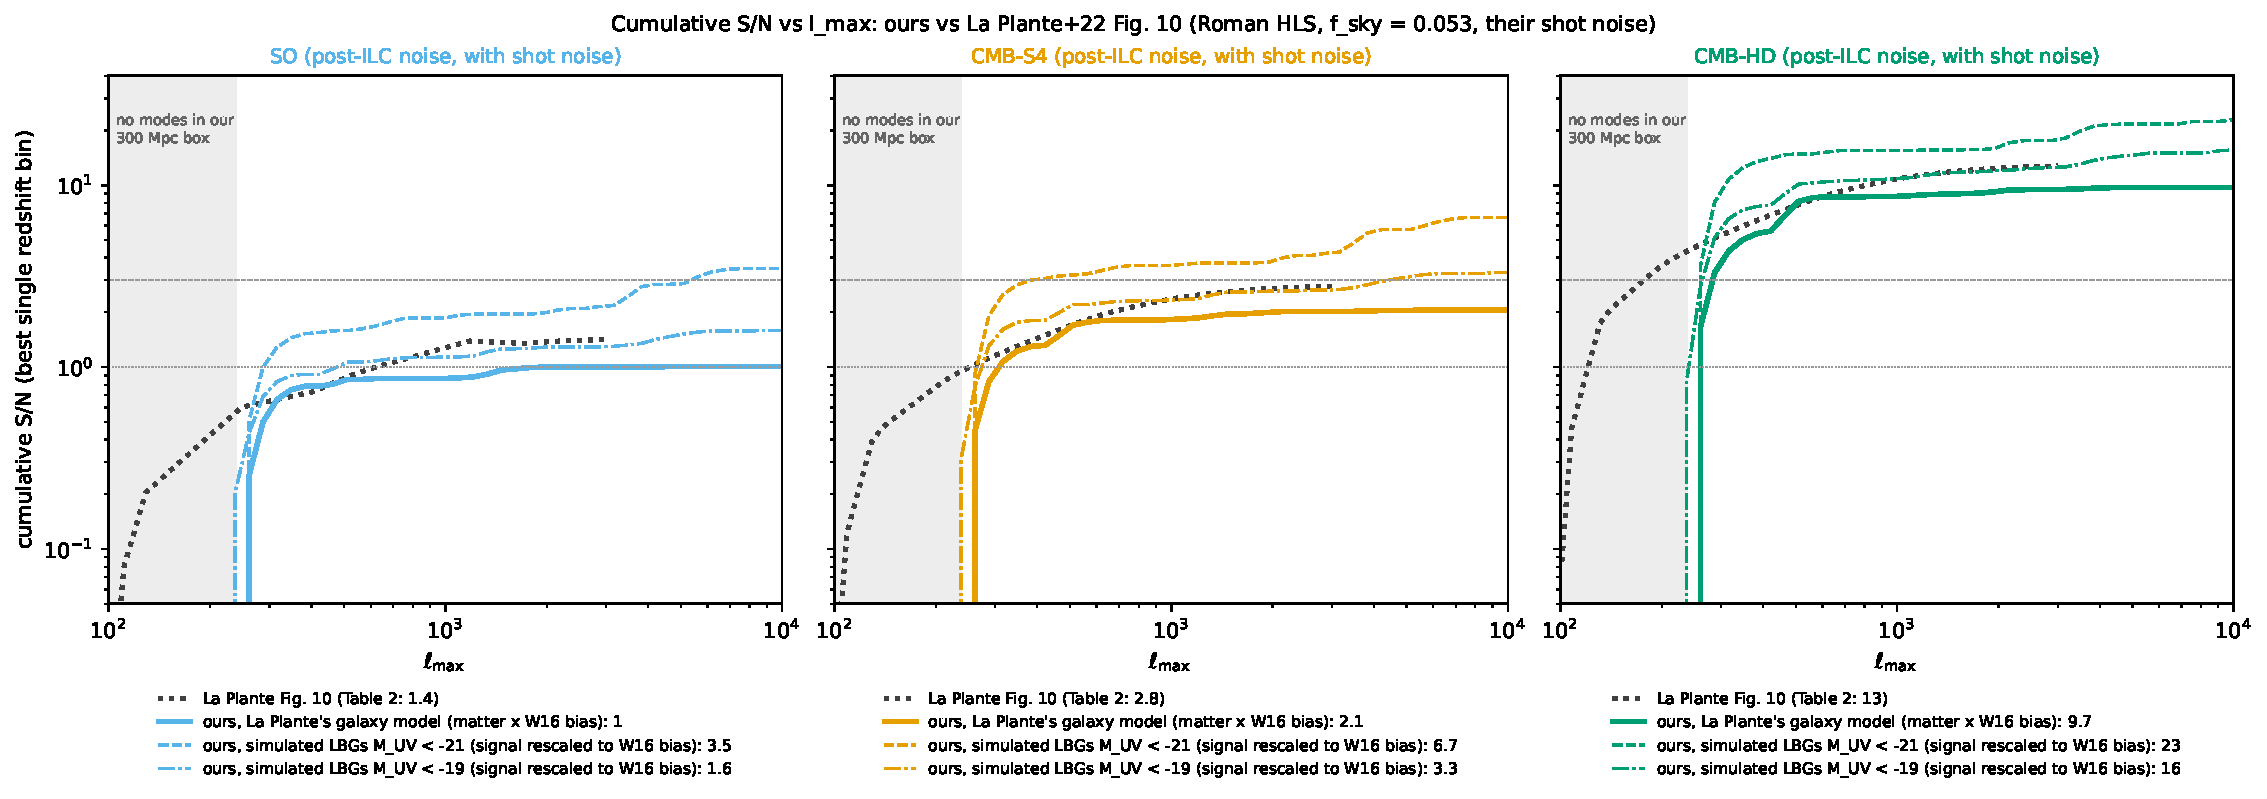
\includegraphics[width=\textwidth]{lp_validation/lp_validation_cumulative.pdf}
\caption{Cumulative S/N vs $\ell_{\max}$ for SO, CMB-S4 and CMB-HD (post-ILC noise, with shot noise). Solid: ours (matter $\times$ W16 bias); dotted: \LP\ Fig.~10; dashed and dot-dashed: our simulated LBGs ($M_{\rm UV}<-21$, $<-19$), with the signal rescaled to the W16 bias. Grey band: no modes in our 300\,Mpc box. Right panel: totals vs Table~2.}
\label{fig:cum}
\end{figure}

\begin{figure}[H]\centering
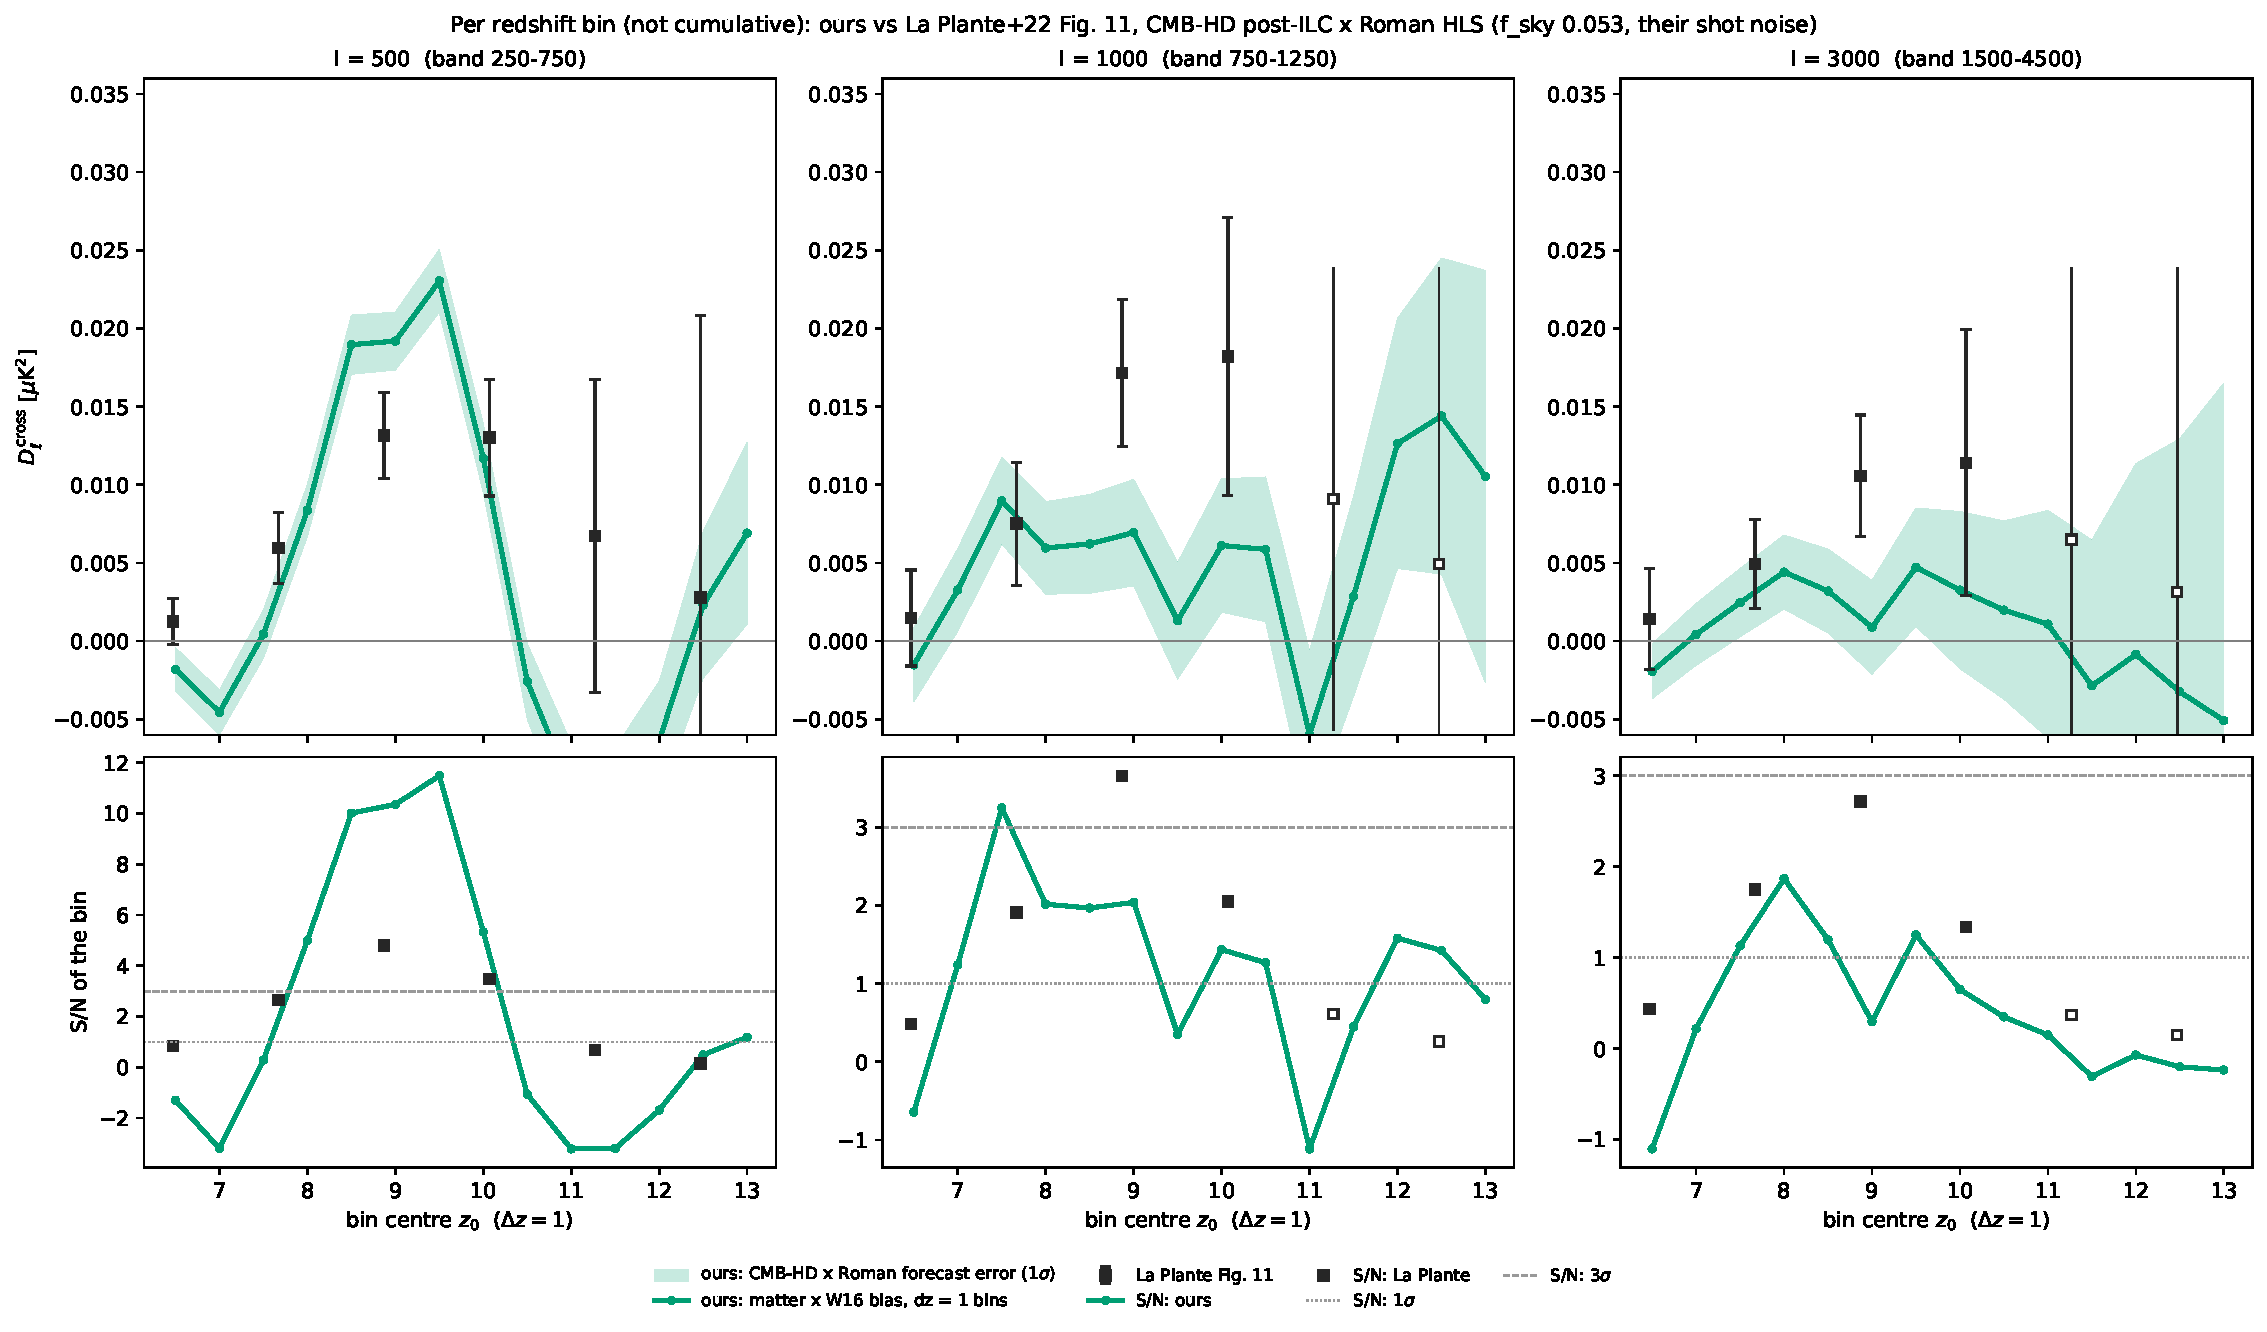
\includegraphics[width=\textwidth]{lp_validation/lp_validation_per_bin.pdf}
\caption{Per redshift bin ($\Delta z=1$), CMB-HD post-ILC $\times$ Roman HLS: our $D_\ell$ with forecast errors (green) vs \LP\ Fig.~11 (black; open squares: error bar runs off their axis), in their three $\ell$ bands. Bottom row: S/N of each bin.}
\label{fig:perbin}
\end{figure}

\begin{figure}[H]\centering
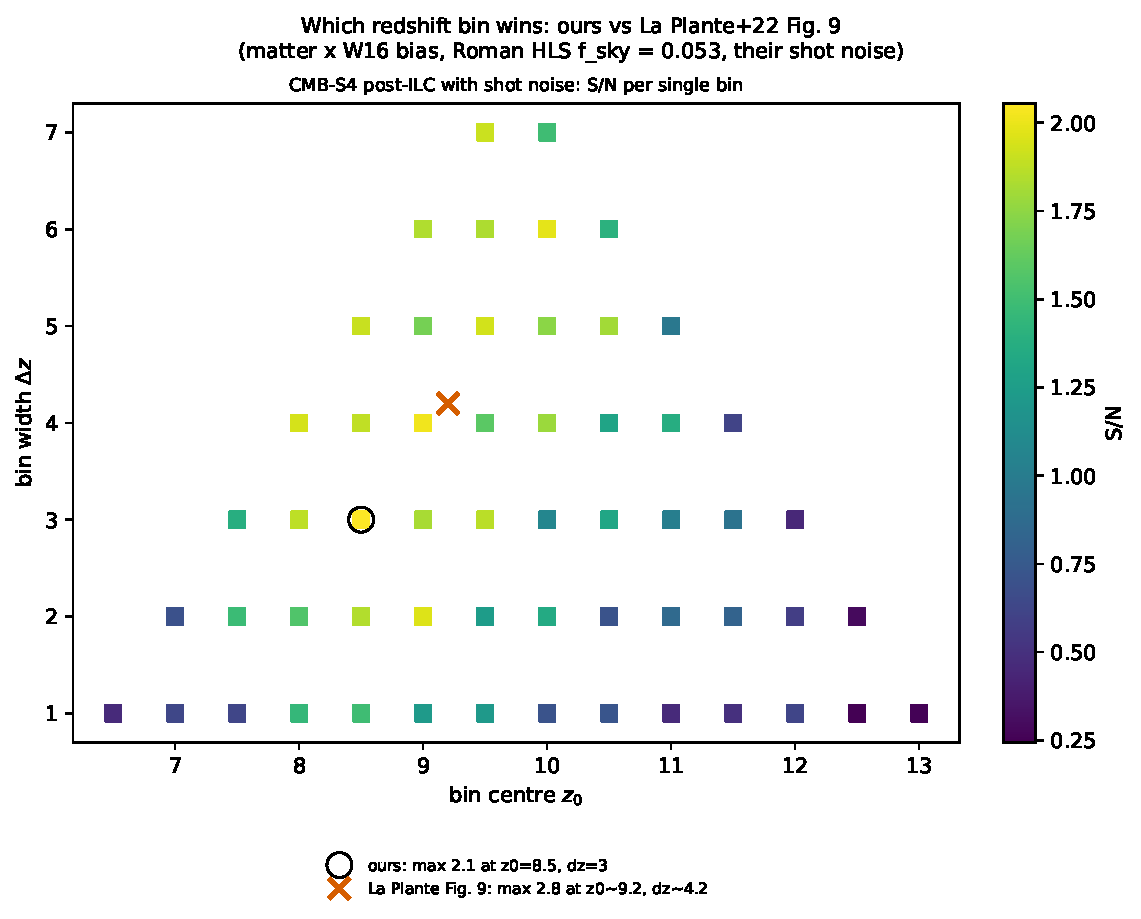
\includegraphics[width=0.55\textwidth]{lp_validation/lp_validation_best_bin.pdf}
\caption{S/N of every single redshift bin $(z_0,\Delta z)$ for CMB-S4 (post-ILC, with shot noise), the analogue of \LP\ Fig.~9. Circle: our best bin; cross: theirs.}
\label{fig:bestbin}
\end{figure}

\paragraph{Findings.}
\begin{itemize}
\item \textbf{Clustering.} Our galaxy clustering matches \LP\ Fig.~8 to $\sim$5\% ($D^{gg}_{1000}=0.16$, 0.21, 0.26, 0.28 at $z_0=7$--10).
\item \textbf{Noise.} Our per-bin errors at $\ell\approx1000$ and 3000 match their Fig.~11, so the noise side of the pipeline (filter, CMB noise, shot noise, sample variance) is validated.
\item \textbf{Best bin.} The best single bin lies in the same region (ours $z_0=8.5$, $\Delta z=3$; theirs $z_0\approx9.2$, $\Delta z\approx4.2$).
\item \textbf{Large scales.} Our box has no modes below $\ell\approx240$. In their Fig.~10, for CMB-HD, 4.3 of the 12.8 total S/N comes from below that $\ell$.
\item \textbf{Signal amplitude.} Our signal at $\ell\gtrsim1000$ is $\sim$0.4--0.5 of theirs near the peak. Likely causes are the box size (missing large-scale velocity modes) and our weaker simulated kSZ; the reionisation histories are similar ($x_{\rm HII}\approx0.19$ vs 0.20 at $z=9$). Our $\ell\approx500$ band is unreliable: it contains only $\sim$2 Fourier modes of a 300\,Mpc patch.
\item \textbf{Open.} Their ``without shot noise'' totals are far above their ``with'' totals, while ours barely change; this is not understood yet.
\end{itemize}

\section{Detectability for the requested CMB$\times$LAE pairs}\label{sec:pairs}
The pairs are: (1) existing data, ACT DR6 $\times$ HSC SILVERRUSH ($z\approx6.6$); (2) a better CMB with the same LAEs, SO LAT $\times$ SILVERRUSH and SO LAT $\times$ LAGER ($z\approx6.9$); (3) better LAEs, SO LAT $\times$ a deep Roman grism field ($z\approx7.5$--10); (4) both better, CMB-HD $\times$ Roman deep. We also show SPT-3G $\times$ SILVERRUSH as a hypothetical (no real overlap). Scripts 58 and 59.

\begin{table}[H]\centering\small
\resizebox{\textwidth}{!}{\begin{tabular}{lllcccc}
\toprule
pair & CMB (noise) & LAE survey & LAEs/deg$^2$ & S/N, LP22 galaxy model & S/N, sim.\ LAEs & area for 3$\sigma$ [deg$^2$] \\
\midrule
1 & ACT DR6 (white noise) & HSC SILVERRUSH & 41 & 0.0074 & 0.0159 & $>$ full sky \\
1s & SPT-3G Main (white noise) & HSC SILVERRUSH $^\dagger$ & 41 & 0.0619 & 0.1066 & $>$ full sky \\
2a & SO (post-ILC) & HSC SILVERRUSH & 41 & 0.0054 & 0.0118 & $>$ full sky \\
2a & SO (white noise) & HSC SILVERRUSH & 41 & 0.007 & 0.015 & $>$ full sky \\
2b & SO (post-ILC) & LAGER & 17 & 0.0031 & 0.0112 & $>$ full sky \\
2b & SO (white noise) & LAGER & 17 & 0.004 & 0.0143 & $>$ full sky \\
3 & SO (post-ILC) & Roman deep (no LF evol.) & 124 / 112 / 52 & 0.0068 & 0.0659 & $>$ full sky \\
3 & SO (white noise) & Roman deep (no LF evol.) & 124 / 112 / 52 & 0.0088 & 0.0855 & $>$ full sky \\
3 & SO (post-ILC) & Roman deep (LF as obs.) & 11 / 10 / 5 & 0.0029 & 0.0267 & $>$ full sky \\
3 & SO (white noise) & Roman deep (LF as obs.) & 11 / 10 / 5 & 0.0037 & 0.0342 & $>$ full sky \\
4 & CMB-HD (post-ILC) & Roman deep (no LF evol.) & 124 / 112 / 52 & 0.0833 & 0.4678 & 1.3e+03 \\
4 & CMB-HD (white noise) & Roman deep (no LF evol.) & 124 / 112 / 52 & 0.2156 & 1.171 & 194 \\
4 & CMB-HD (post-ILC) & Roman deep (LF as obs.) & 11 / 10 / 5 & 0.0361 & 0.2179 & 6.9e+03 \\
4 & CMB-HD (white noise) & Roman deep (LF as obs.) & 11 / 10 / 5 & 0.0933 & 0.5817 & 1.03e+03 \\
\bottomrule
\multicolumn{7}{l}{\footnotesize $^\dagger$ SPT-3G Main and SILVERRUSH do not overlap on the sky; computed as if they did (real S/N = 0).} \\
\end{tabular}
}
\caption{S/N for each pair (all $\ell$, all shells of the survey; seed scatter removed). The LAEs/deg$^2$ column gives the value per shell. The 3$\sigma$ area assumes the same depth and density.}
\label{tab:pairs}
\end{table}

\begin{figure}[H]\centering
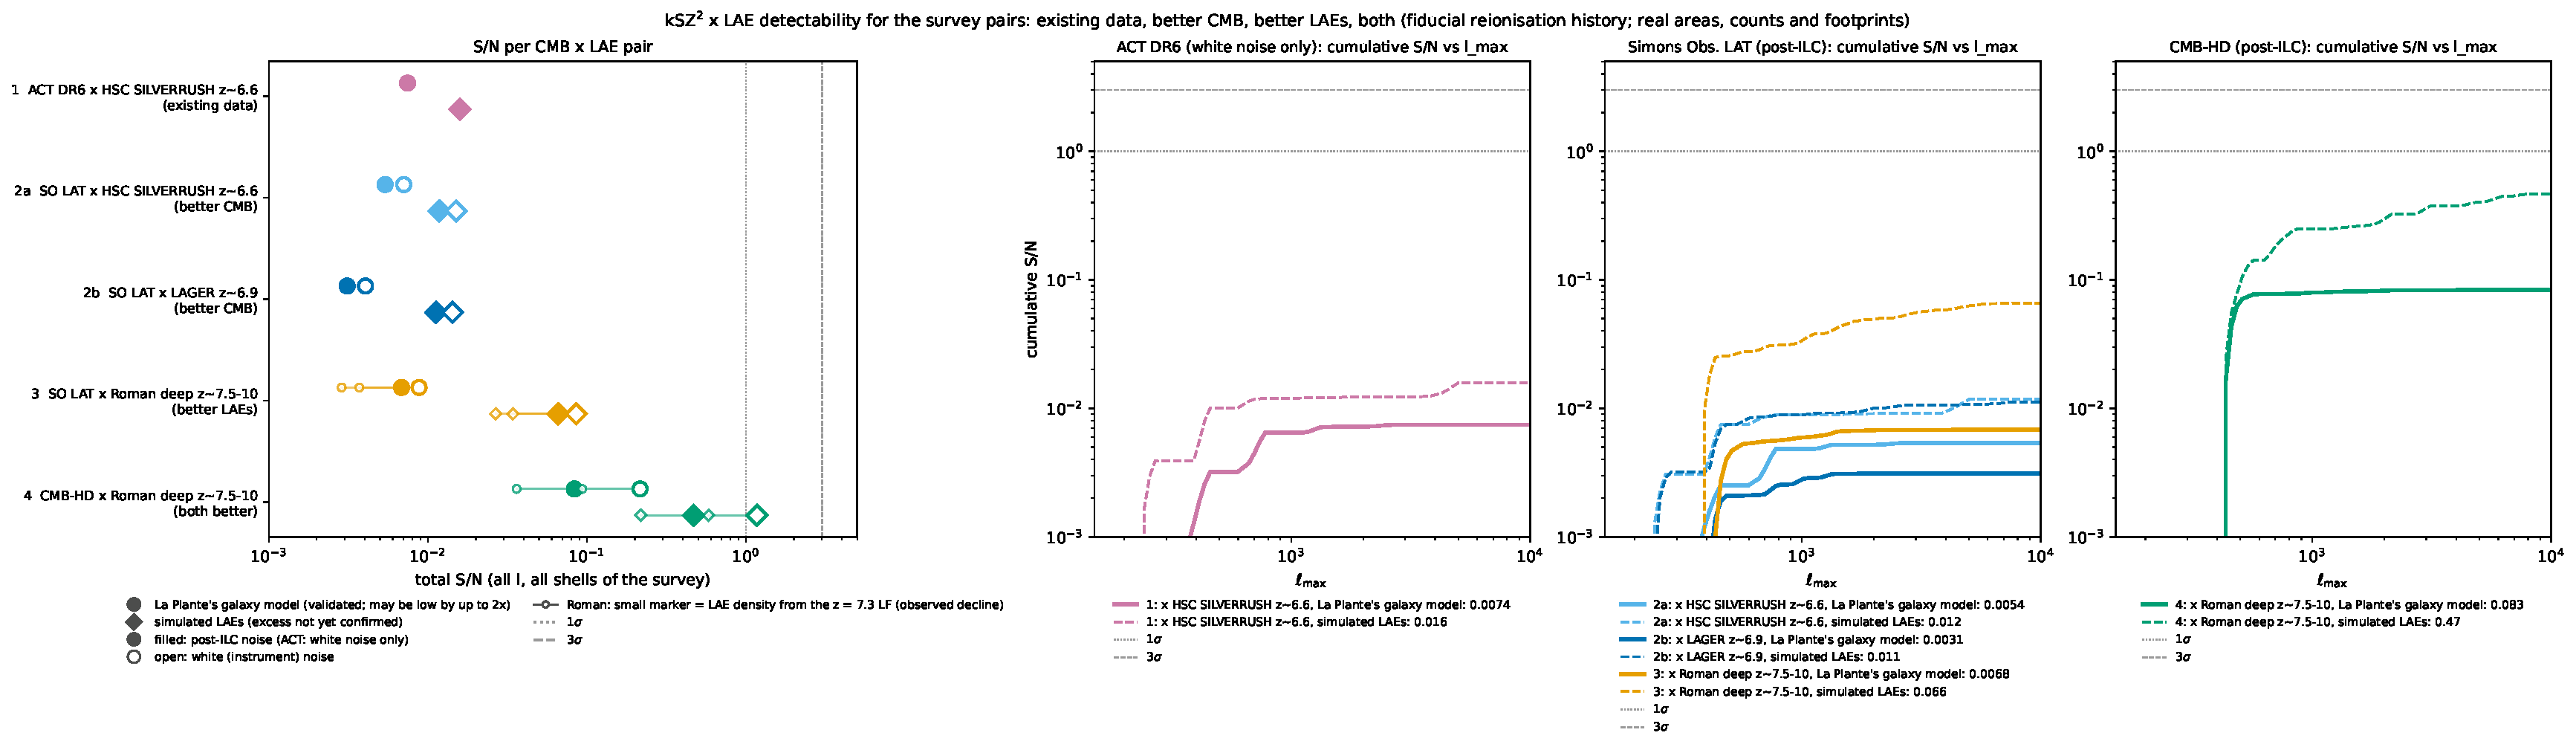
\includegraphics[width=\textwidth]{detectability_pairs/detectability_pairs.pdf}
\caption{Left: total S/N per pair. Circles: La~Plante's galaxy model (validated); diamonds: simulated LAEs. Filled: post-ILC noise (ACT, SPT-3G: white noise only); open: white noise. For Roman, the small marker uses the $z=7.3$ LF. Right: cumulative S/N vs $\ell_{\max}$, one panel per CMB experiment.}
\label{fig:pairs}
\end{figure}

\paragraph{Per-pair curves.} Figures~\ref{fig:pair1}--\ref{fig:pair4} show one pair each. Left: the S/N if the survey (same area, density, depth and shell width) sat at each $\Delta z=1$ window; stars mark its real shells. Right: cumulative S/N for the real shells. Solid: simulated LAEs; dashed: La~Plante's galaxy model; thick: post-ILC; thin: white noise. Grey band: the LAE bias is held constant beyond the measured redshift.

\begin{figure}[H]\centering
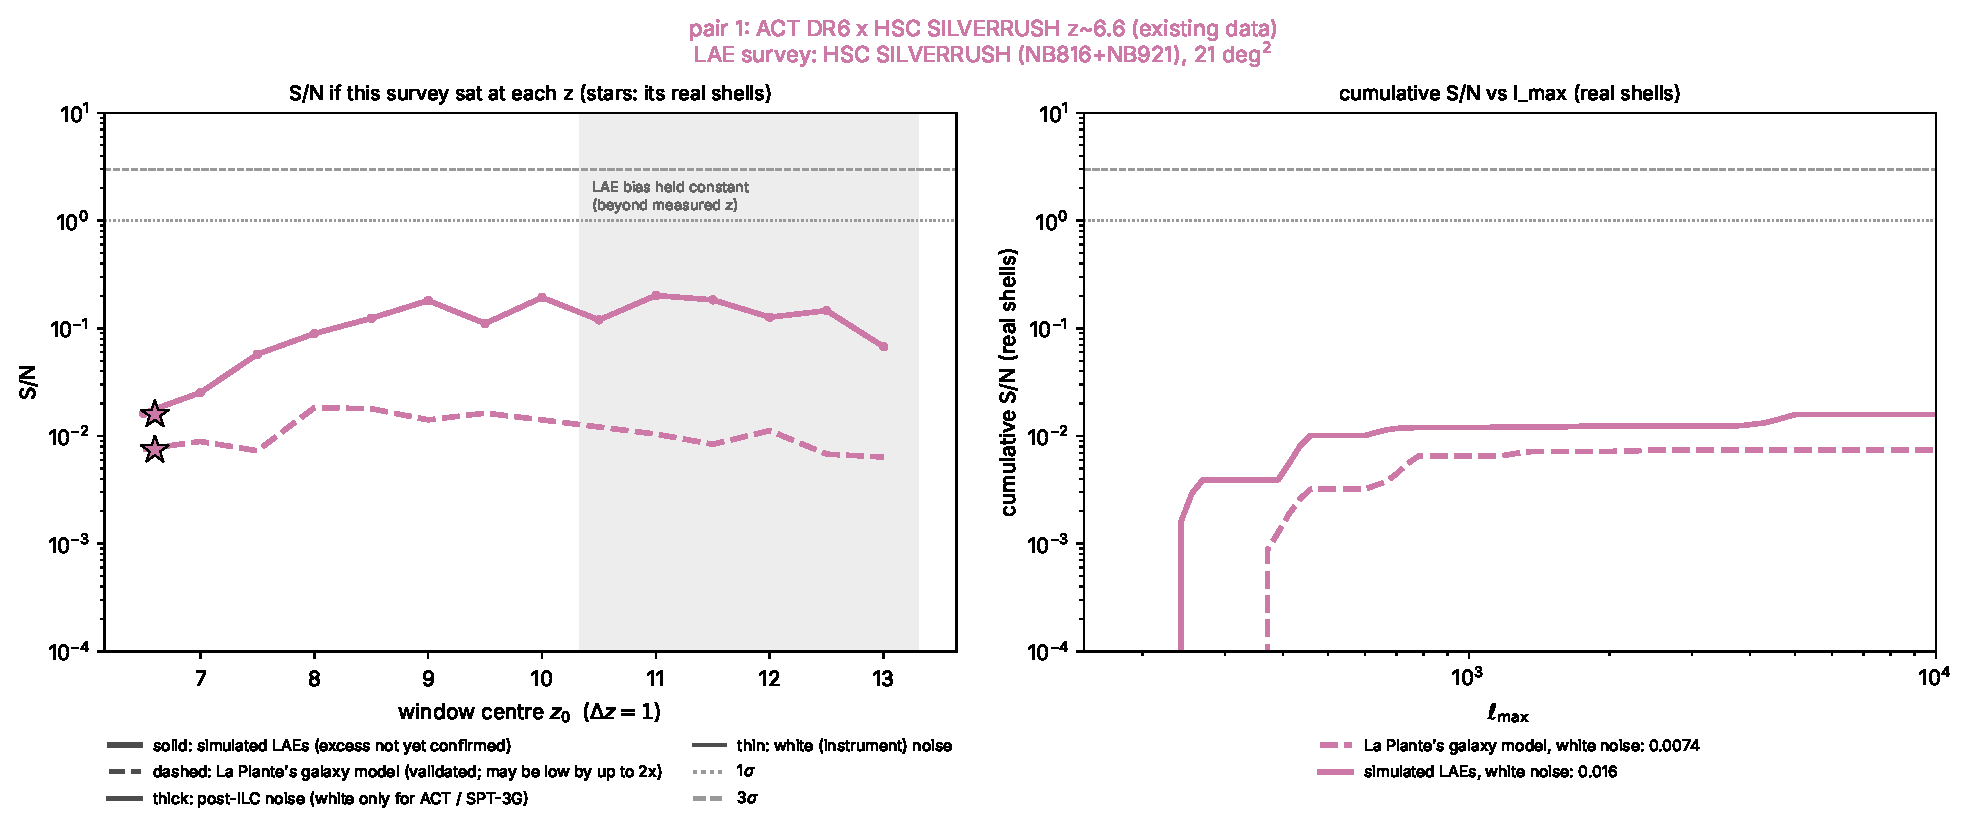
\includegraphics[width=0.92\textwidth]{detectability_pairs/pair_1.pdf}
\caption{Pair 1: ACT DR6 $\times$ HSC SILVERRUSH ($z\approx6.6$), existing data.}
\label{fig:pair1}
\end{figure}

\begin{figure}[H]\centering
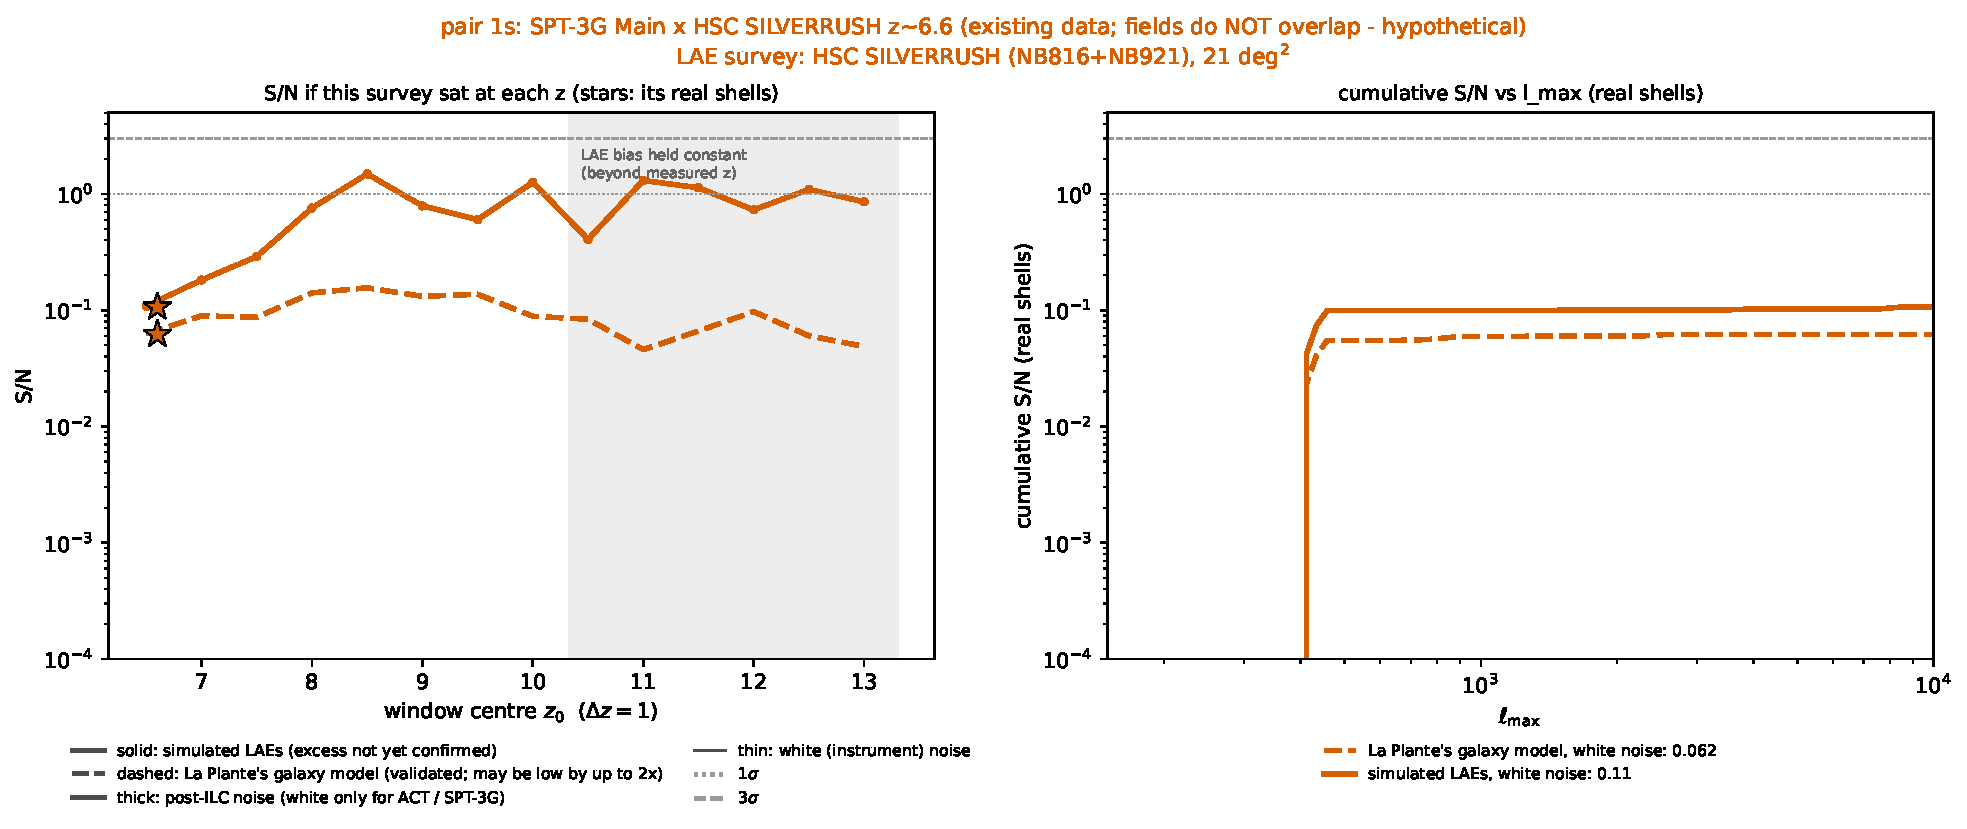
\includegraphics[width=0.92\textwidth]{detectability_pairs/pair_1s.pdf}
\caption{Pair 1s: SPT-3G Main $\times$ HSC SILVERRUSH, hypothetical (the fields do not overlap).}
\label{fig:pair1s}
\end{figure}

\begin{figure}[H]\centering
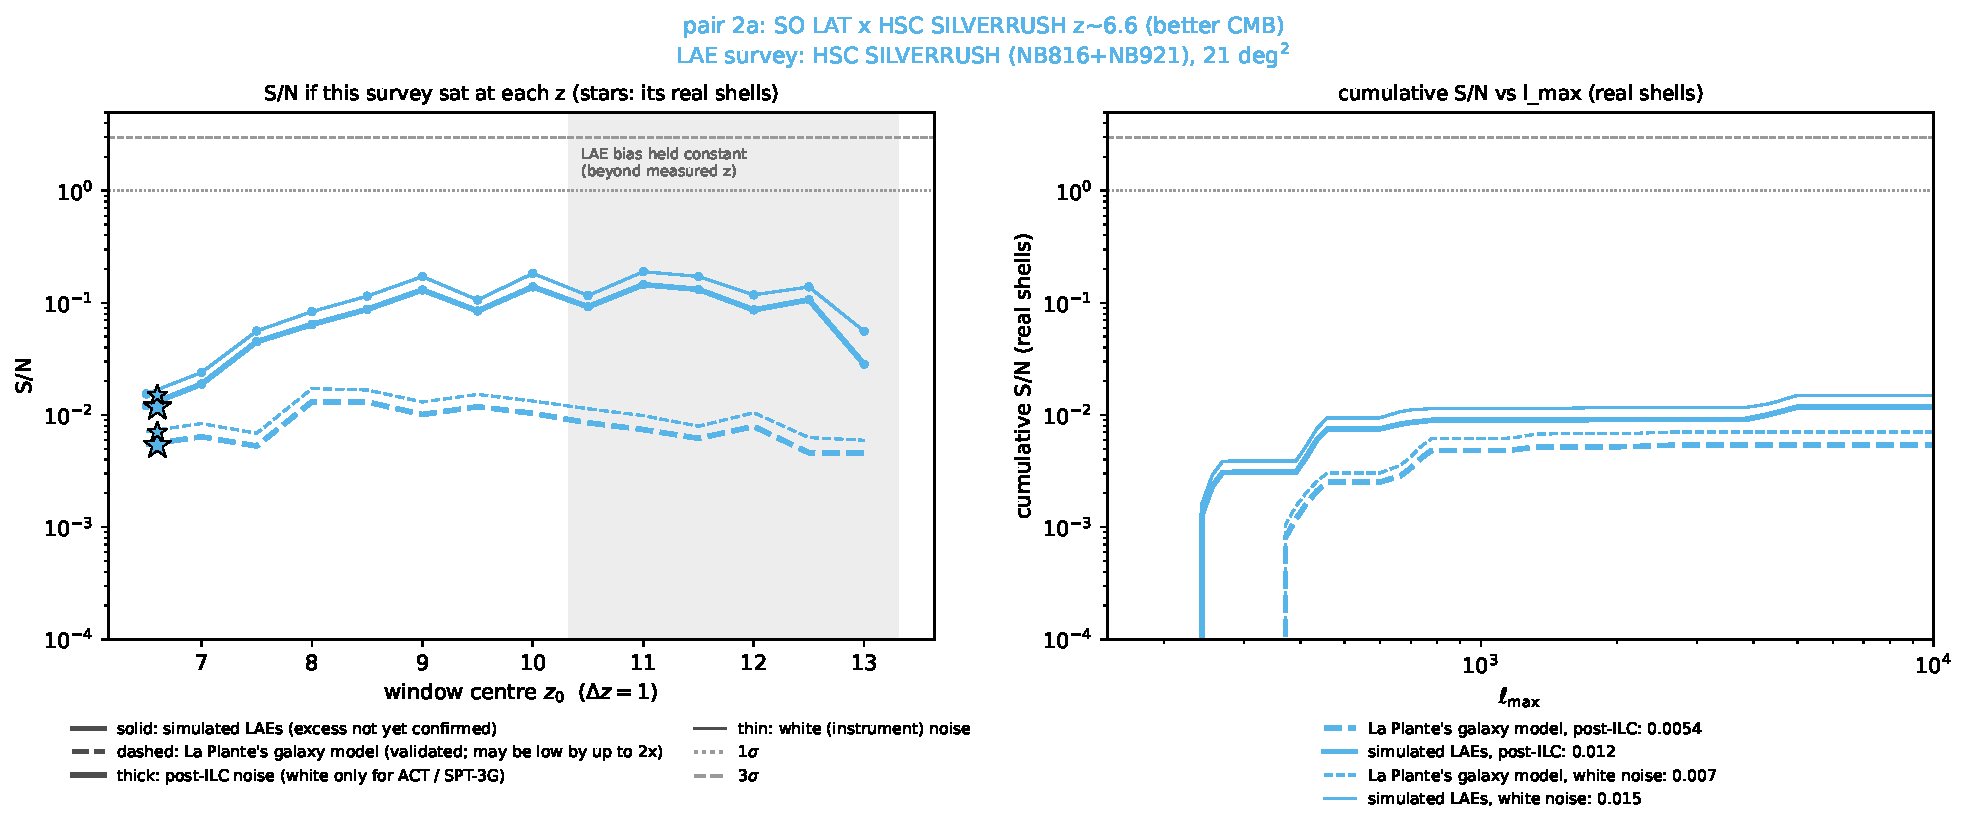
\includegraphics[width=0.92\textwidth]{detectability_pairs/pair_2a.pdf}
\caption{Pair 2a: SO LAT $\times$ HSC SILVERRUSH ($z\approx6.6$), better CMB.}
\label{fig:pair2a}
\end{figure}

\begin{figure}[H]\centering
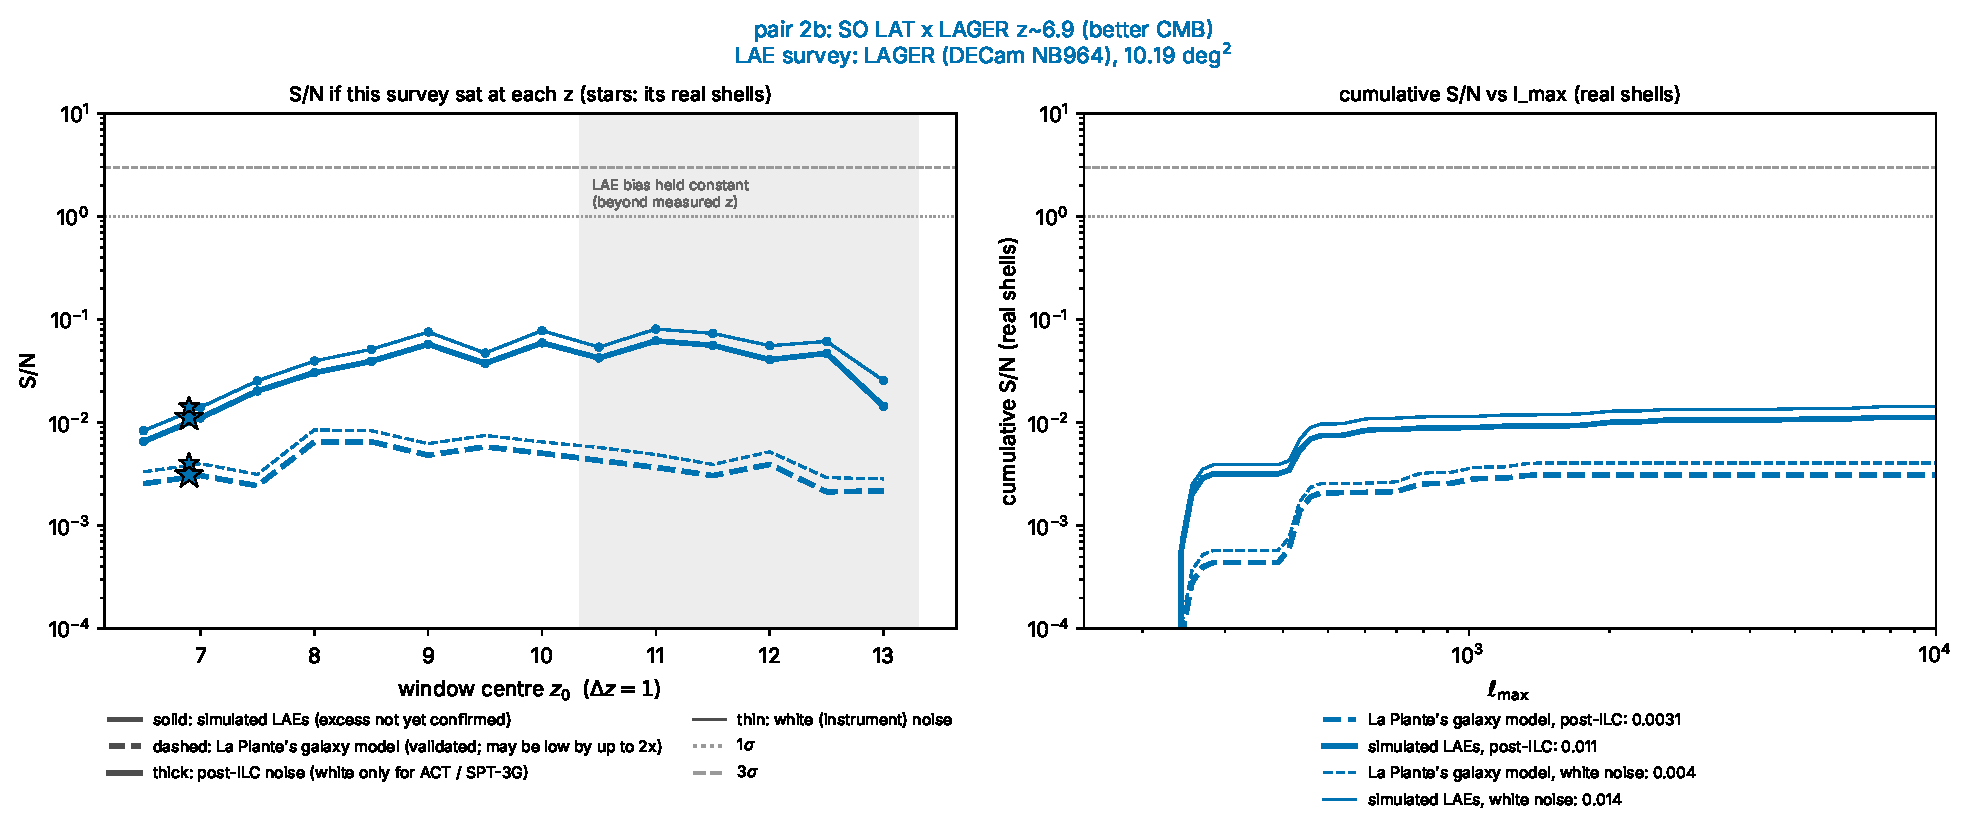
\includegraphics[width=0.92\textwidth]{detectability_pairs/pair_2b.pdf}
\caption{Pair 2b: SO LAT $\times$ LAGER ($z\approx6.9$), better CMB.}
\label{fig:pair2b}
\end{figure}

\begin{figure}[H]\centering
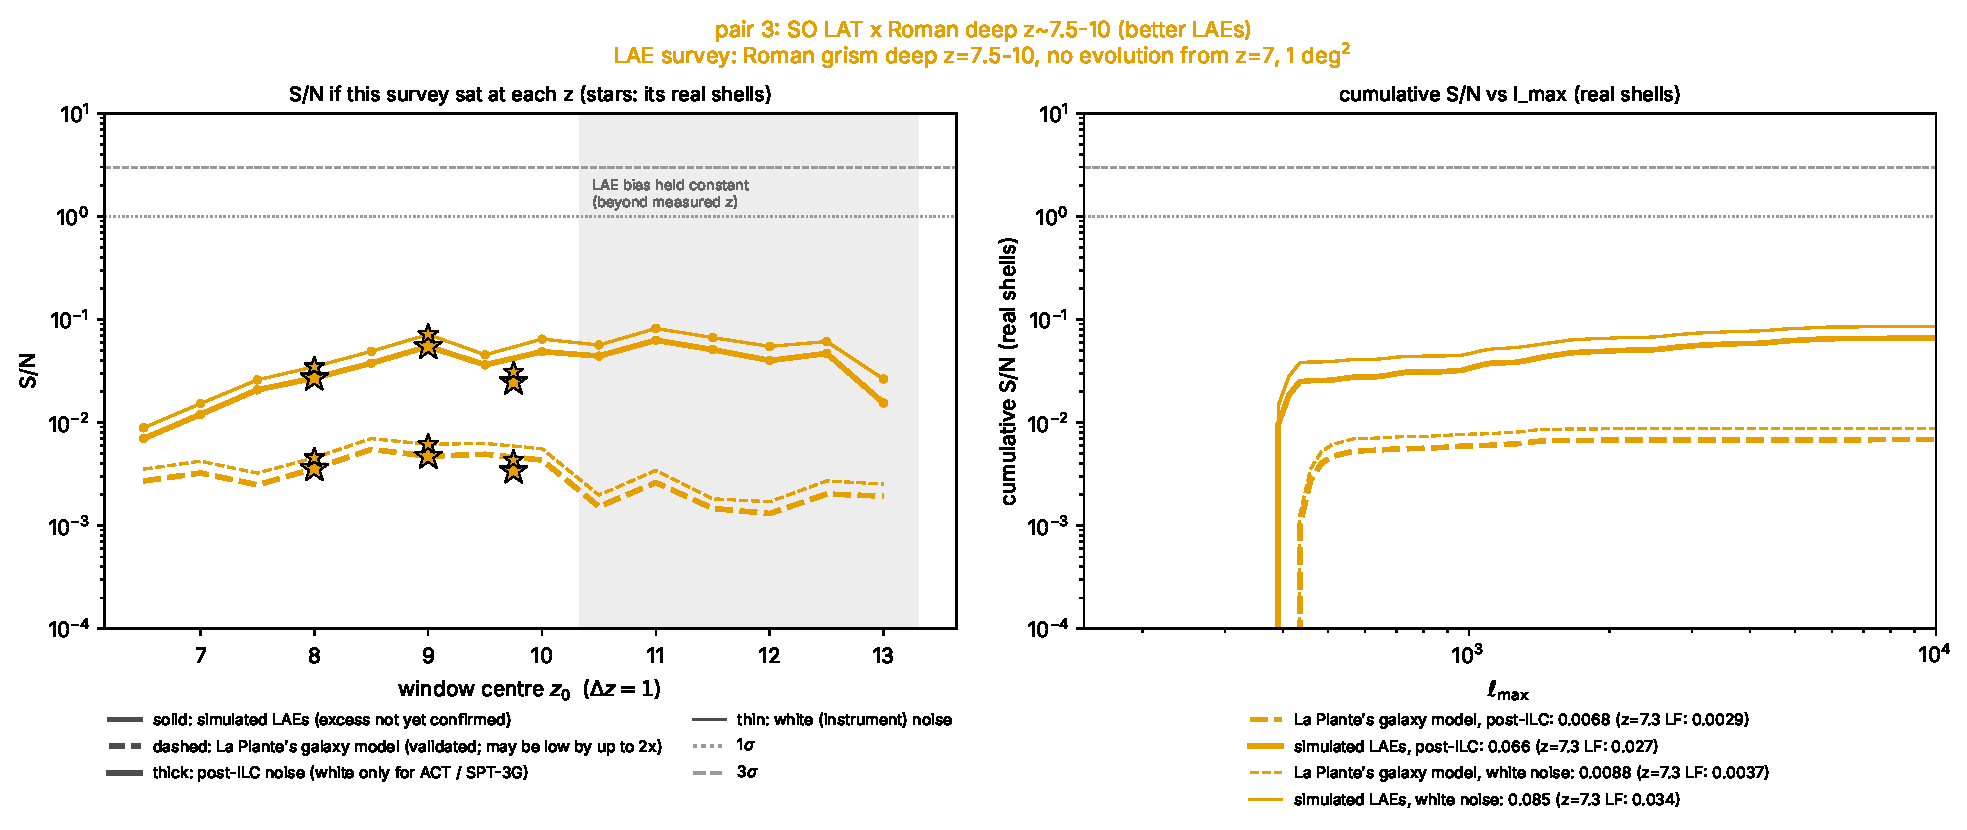
\includegraphics[width=0.92\textwidth]{detectability_pairs/pair_3.pdf}
\caption{Pair 3: SO LAT $\times$ Roman deep ($z\approx7.5$--10), better LAEs.}
\label{fig:pair3}
\end{figure}

\begin{figure}[H]\centering
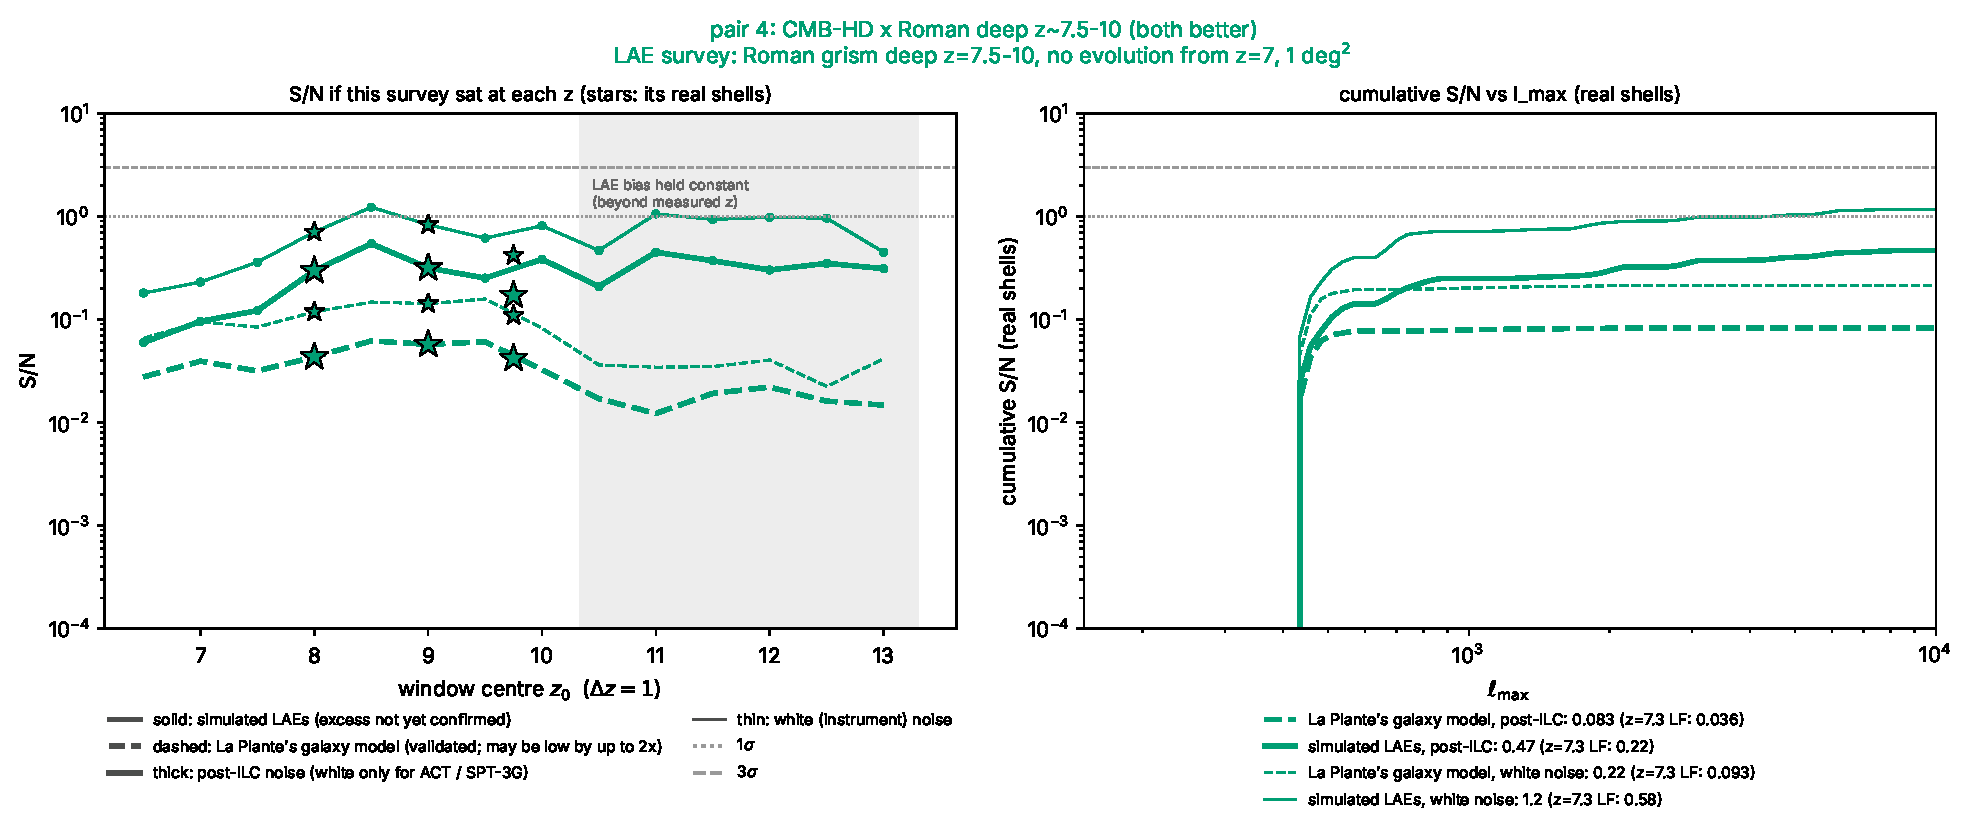
\includegraphics[width=0.92\textwidth]{detectability_pairs/pair_4.pdf}
\caption{Pair 4: CMB-HD $\times$ Roman deep ($z\approx7.5$--10), both better.}
\label{fig:pair4}
\end{figure}



\paragraph{Reading.}
\begin{itemize}
\item \textbf{Existing data} give S/N $\sim$0.01.
\item \textbf{SO LAT} has a map depth similar to ACT DR6 (10 vs 9.6\,$\mu$K-arcmin), and its larger sky area does not help a 10--20\,deg$^2$ LAE field.
\item \textbf{SPT-3G}'s much deeper map would give $\sim$8$\times$ ACT on the same field, if an LAE field existed inside its footprint.
\item \textbf{Redshift.} The $z\approx6.6$--6.9 surveys sit where the signal has mostly faded; the signal peaks at $z\approx8$--9, where Roman observes.
\item \textbf{Area.} Only CMB-HD $\times$ Roman approaches 1$\sigma$. The limit is the LAE survey area.
\end{itemize}

\section{All surveys $\times$ all CMB experiments}
For completeness (CMB-S4 kept for comparison only), script 55:
\begin{figure}[H]\centering
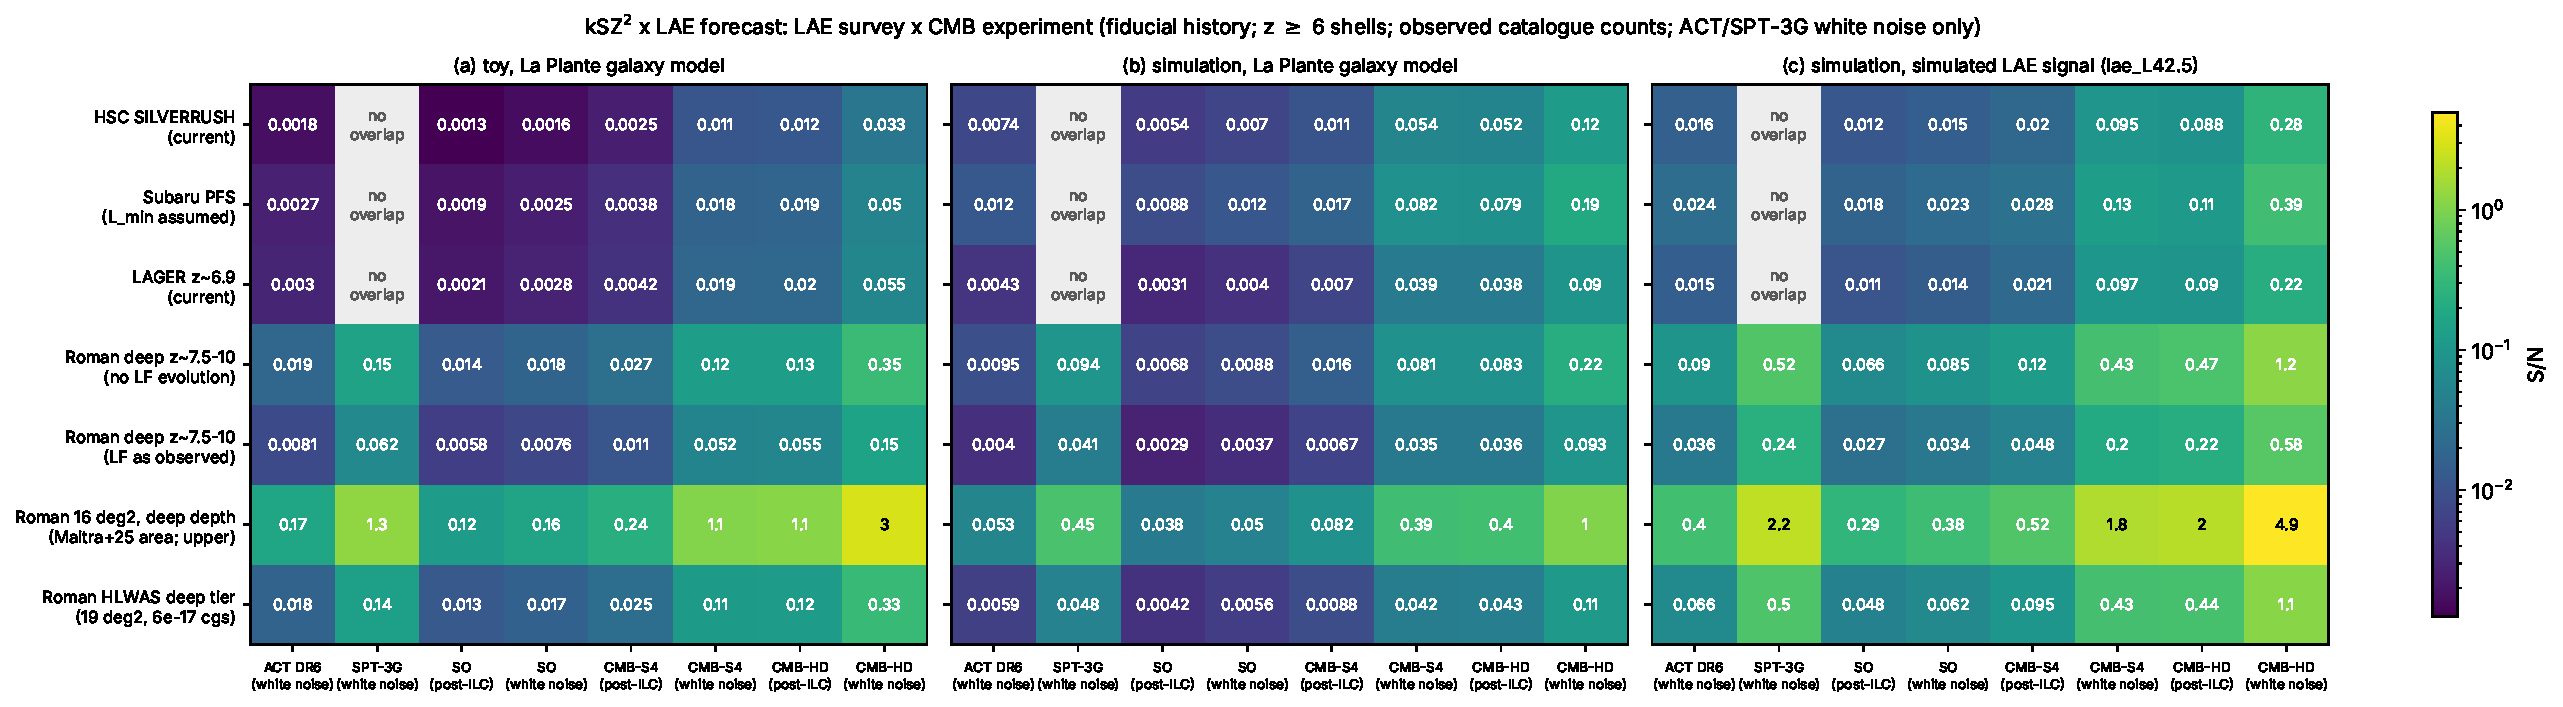
\includegraphics[width=\textwidth]{survey_forecast/survey_forecast.pdf}
\caption{S/N for every LAE survey (rows) and CMB experiment (columns). (a) the toy model calibrated to \LP\ Table~2 (one rescaling factor, 1.45); (b) the simulation with La~Plante's galaxy model; (c) the simulation with the simulated LAEs. Only shells at $z\ge6$ are used (the simulation starts at $z=5$, and the kSZ map at $z=6$).}
\label{fig:heat}
\end{figure}
\begin{table}[H]\centering\small
\resizebox{\textwidth}{!}{\begin{tabular}{lcccccccc}
\toprule
survey / signal & \shortstack{ACT DR6\\(white noise)} & \shortstack{SPT-3G\\(white noise)} & \shortstack{SO\\(post-ILC)} & \shortstack{SO\\(white noise)} & \shortstack{CMB-S4\\(post-ILC)} & \shortstack{CMB-S4\\(white noise)} & \shortstack{CMB-HD\\(post-ILC)} & \shortstack{CMB-HD\\(white noise)} \\
\midrule
HSC SILVERRUSH, LP22 model & 0.0074 & -- & 0.0054 & 0.007 & 0.011 & 0.054 & 0.052 & 0.12 \\
HSC SILVERRUSH, sim. LAEs & 0.016 & -- & 0.012 & 0.015 & 0.02 & 0.095 & 0.088 & 0.28 \\
Subaru PFS, LP22 model & 0.012 & -- & 0.0088 & 0.012 & 0.017 & 0.082 & 0.079 & 0.19 \\
Subaru PFS, sim. LAEs & 0.024 & -- & 0.018 & 0.023 & 0.029 & 0.13 & 0.11 & 0.39 \\
LAGER, LP22 model & 0.0043 & -- & 0.0031 & 0.004 & 0.007 & 0.039 & 0.038 & 0.09 \\
LAGER, sim. LAEs & 0.015 & -- & 0.011 & 0.014 & 0.021 & 0.097 & 0.09 & 0.22 \\
Roman deep (no LF evol.), LP22 model & 0.0095 & 0.094 & 0.0068 & 0.0088 & 0.016 & 0.081 & 0.083 & 0.22 \\
Roman deep (no LF evol.), sim. LAEs & 0.09 & 0.52 & 0.066 & 0.086 & 0.12 & 0.43 & 0.47 & 1.2 \\
Roman deep (LF as obs.), LP22 model & 0.004 & 0.041 & 0.0029 & 0.0037 & 0.0067 & 0.035 & 0.036 & 0.093 \\
Roman deep (LF as obs.), sim. LAEs & 0.036 & 0.24 & 0.027 & 0.034 & 0.048 & 0.2 & 0.22 & 0.58 \\
\bottomrule
\end{tabular}
}
\caption{The numbers of Fig.~\ref{fig:heat}(b, c). ``--'': no footprint overlap.}
\label{tab:heat}
\end{table}

\section{Caveats and open items}
\begin{itemize}
\item \textbf{Noise model.} Gaussian covariance as in \LP. Super-sample variance, non-Gaussian kSZ$^2$ covariance and the real field geometry are not included; all of them would lower the S/N of the small LAE fields.
\item \textbf{ACT and SPT-3G}: instrument noise only (no foreground residuals), so optimistic.
\item \textbf{Signal amplitude.} Up to $\sim$2$\times$ below \LP\ at $\ell\gtrsim1000$; a bigger box is needed (the planned large-box LAE runs with Jahaan).
\item \textbf{Simulated-LAE excess.} Not yet confirmed. Next: a mismatched-seed null test and a halo sample matched in number density.
\item \textbf{Survey bias.} Abundance matching without scatter, so an upper value. PFS $L_{\min}$ is assumed. The Roman density is bracketed by two LF choices.
\item \textbf{Footprints.} ELAIS-N1 is not removed from SILVERRUSH; the Roman deep-field position is assumed inside the CMB footprint.
\end{itemize}

\section*{Reproducing the numbers}\sloppy
Repository \texttt{ksz-lae-xcorr}. Script 53 (on the cluster) writes the binned spectra \texttt{data/products\_tracers/sim\_spectra/*.npz}; scripts 55, 57, 58 and 59 (on a desktop, seconds to minutes) write the figures and CSVs under \texttt{data/plots/2026-11-03\_ksz\_lae\_snr/}; script 60 writes the tables of this report. The code is \texttt{src/ksz\_lae\_xcorr/snr/feasibility.py} (experiments, surveys, filter, bias) and \texttt{snr/sim\_snr.py} (estimator on the simulated spectra).

\section*{References}
\small
\begin{itemize}\setlength\itemsep{1pt}
\item CASCA GAC report to the CASCA Board, Dec.\ 2025 (CMB-S4 status), \href{https://casca.ca/wp-content/uploads/2026/03/GAC-Report-to-CASCA-Board-December-2025-2.pdf}{casca.ca}
\item Davies, Mesinger, Murray et al.\ 2025, 21cmFAST v4, arXiv:2504.17254
\item Eisenstein \& Hu 1998, arXiv:astro-ph/9709112
\item Ferraro et al.\ 2016 (projected-field kSZ estimator; via \LP)
\item Konno et al.\ 2018, SILVERRUSH IV, arXiv:1705.01222
\item La~Plante, Sipple \& Lidz 2022, ApJ 928, 162, arXiv:2111.13717 (\LP)
\item Mesinger, Furlanetto \& Cen 2011, 21cmFAST, arXiv:1003.3878
\item Naess et al.\ 2025, ACT DR6 maps, arXiv:2503.14451
\item Ouchi et al.\ 2018, SILVERRUSH I, arXiv:1704.07455
\item Park et al.\ 2018 (late-time kSZ; via \LP\ Eq.~9), arXiv:1710.02792
\item Sheth \& Tormen 1999, arXiv:astro-ph/9901122
\item Sheth, Mo \& Tormen 2001, MNRAS 323, 1, arXiv:astro-ph/9907024
\item Simons Observatory collaboration 2019, science goals, arXiv:1808.07445
\item SPT-3G collaboration 2024, arXiv:2403.17925
\item Umeda et al.\ 2025, SILVERRUSH XIV, arXiv:2411.15495
\item Waters et al.\ 2016, MNRAS 463, 3520, arXiv:1605.05670
\item Weinberger, Kulkarni \& Haehnelt 2020, arXiv:1911.11783
\item Wold et al.\ 2022, LAGER Ly$\alpha$ LF at $z\sim7$, arXiv:2105.12191
\item Wold et al.\ 2023, Roman grism deep field, arXiv:2305.01562
\end{itemize}
\end{document}
